%!TEX root = ../thesis.tex
%*******************************************************************************
%*********************************** Analysis Overview *********
%*******************************************************************************

\chapter{Analysis overview}\label{ch:1lepton}

\ifpdf
    \graphicspath{{chapter-analysis/Figs/Raster/}{chapter-analysis/Figs/PDF/}{chapter-analysis/Figs/}}
\else
    \graphicspath{{chapter-analysis/Figs/Vector/}{chapter-analysis/Figs/}}
\fi


This chapter aims to give an introduction to the search for electroweakinos presented in this work. First, the targeted final state, the 1-lepton final state, is introduced and motivated, followed by the \gls{sm} background processes that need to be considered when doing searches for \gls{susy} in this final state. Next the reconstruction and identification of physics objects as well as the event selection requirements are described.

\section{Search for electroweakinos in the 1-lepton final state}

In the search for electroweakinos presented herein, the simplified model introduced in \cref{sec:models_used} is interpreted in final states with one lepton, two \textit{b}-jets and high missing transverse momentum. This final state can occur when the $W$ boson decays through $W^\pm\rightarrow\ell^\pm\nu_\ell$, while the Higgs boson decays into $h\rightarrow b\bar{b}$. Although a final state without leptons would benefit from the higher branching fraction of the $W^\pm\rightarrow q'\bar{q}$ decay, due to the \gls{qcd} couplings these final states are largely dominated by \gls{qcd} multi-jet background processes that are omnipresent at hadron colliders like the \gls{lhc}. Final states with exactly one lepton have lower cross sections but allow to reject a majority of the \gls{qcd} background, as pure \gls{qcd} multi-jet events can only appear in the 1-lepton final state through false reconstruction of a jet as a lepton (so-called \textit{fake} leptons). 

Targeting the decay of the Higgs boson into a pair of \textit{b} quarks benefits from the high branching ratio of 58.3\% and allows a full reconstruction of Higgs candidates, a procedure that will be used to achieve a high signal-to-background ratio. \improvement{refer to observables} \Cref{fig:Wh_model_full} shows the full signal model targeted in this search, including the considered decays of the $W$ and Higgs bosons. 

Previous searches for electroweakinos in this final state have been performed by the ATLAS~\cite{SUSY-2013-23,SUSY-2017-01} and CMS~\cite{CMS-SUS-16-043} collaborations, excluding $\charg\neutr$ masses up to $\SI{540}{\GeV}$ and $\SI{490}{\GeV}$, respectively, for massless $\lsp$. The two previous ATLAS searches used $\SI{20.3}{\per\femto\barn}$ of $\sqrt{s}=\SI{8}{\TeV}$ and $\SI{36.1}{\per\femto\barn}$ of $\sqrt{s}=\SI{13}{\TeV}$ $pp$ collision data, respectively. As opposed to this, the search presented in the following uses the full dataset available from the Run~2 data taking period, amounting to an unprecedented $\SI{139}{\per\femto\barn}$ of $pp$ collision data at $\sqrt{s}=\SI{13}{\TeV}$.

\begin{figure}
	\centering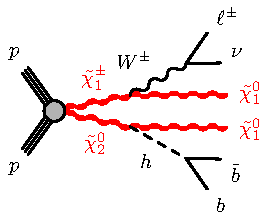
\includegraphics[width=.4\textwidth]{model_c1n2_Wh}
	\caption{Diagram for the simplified model used in this work including the decays $W^\pm\rightarrow\ell^\pm\nu_\ell$ and $h\rightarrow b\bar{b}$.}\label{fig:Wh_model_full}
\end{figure}

\section{Standard Model backgrounds}

Although the requirement of exactly one lepton isolated from surrounding hadronic activity significantly reduces the contribution from \gls{qcd} multi-jet background, numerous \gls{sm} processes can result in final states with exactly one isolated lepton, multiple jets and missing transverse momentum. Background sources are generally classified into \textit{reducible} and \textit{irreducible} backgrounds. Irreducible backgrounds are processes that have a physical phase space that is indistinguishable from the final state of the signal process considered. Reducible backgrounds, on the other hand, result from partially misreconstructed processes as well as mismeasurements. Examples of reducible processes are events where a lepton originates from a \gls{hf} decay, photon conversions or misreconstructed jets. \gls{sm} processes that result in final states with an isolated lepton, multiple jets and missing transverse momentum typically involve a $W$ boson decaying into a lepton--neutrino pair (a so-called \textit{leptonic decay}). The neutrino will contribute to the total missing transverse momentum in the event, while additional jets can appear in the final state through \gls{qcd} radiation or other branches of the decay chain.

By far the largest \gls{sm} background contributions stem from the production of top quarks, predominantly through top quark pair $\ttbar$ production, where both top quarks decay into a $W$ boson and a $b$ quark. Final states with one isolated lepton can occur through leptonic decay of one of the $W$ bosons. \Cref{fig:ttbar} shows a diagram depicting an exemplary decay of a $\ttbar$ system into a final state with one lepton, multiple jets (two of which originate from \textit{b} quarks) and missing transverse momentum. In addition to $\ttbar$, single top production (\textit{s}-channel, \texttt{t}-channel or \textit{tW}-channel) can also result in similar final states as the \gls{susy} signal and thus constitutes a significant \gls{sm} background process. An exemplary decay is shown in~\cref{fig:singletop}.

Apart from processes involving top quarks, the production of a $W$ boson in association with multiple jets ($\wjets$) is the third major background considered in the analysis. If the $W$ boson undergoes a leptonic decay and two of the produced jets are tagged as originating from $b$ quarks, the signature of this process is similar to that of signal events. An exemplary diagram for a $\wjets$ event is shown in~\cref{fig:wjets}. 

Production of multiple vector bosons $V$ ($=W,Z$)---although not a dominant background due to low cross sections---can still result in the same final state as the signal process. In the following, diboson $VV$ and multibosons $VVV$ processes are considered.

Other \gls{sm} backgrounds with small contributions in the phases spaces targeted by the analysis include $Z+\mathrm{jets}$ production, $\ttbar+V$ production, as well as various processes involving Higgs bosons. $Z+\mathrm{jets}$ plays only a minor role, as the only irreducible component is $Z(\rightarrow\tau\tau)+\mathrm{jets}$, where one $\tau$-lepton undergoes a leptonic decay and the other one a hadronic decay. Production of $\ttbar+V$ has a similar topology as ordinary $\ttbar$ processes but with lower cross section and additional objects in the final state. Higgs processes considered in the following include single Higgs production through \gls{vbf} or \gls{ggf} as well as $h+V$ and $h+\ttbar$ processes. In the following, these backgrounds are simply labelled \textit{other}. 

Pure \gls{qcd} multi-jet events can only appear in the 1-lepton final state through false reconstruction of a jet as a lepton (so-called \textit{fake} leptons) and mismeasurement of $\etmiss$. As it has been shown that this background is negligible in all selections relevant to this search, no estimation for \gls{qcd} contribution is considered in the following~\cite{SUSY-2019-08}.

\begin{figure}
	\centering
	\begin{subfigure}[b]{0.3\linewidth}
		\centering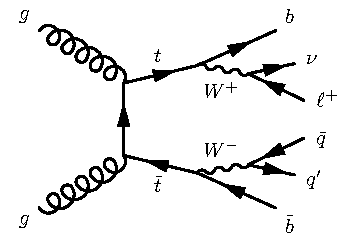
\includegraphics[width=\textwidth]{ttbar}
		\caption{\label{fig:ttbar}}
	\end{subfigure}\quad
		\begin{subfigure}[b]{0.3\linewidth}
		\centering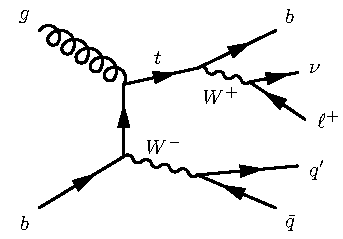
\includegraphics[width=\textwidth]{singletop}
		\caption{\label{fig:singletop}}
	\end{subfigure}\quad
	\begin{subfigure}[b]{0.3\linewidth}
		\centering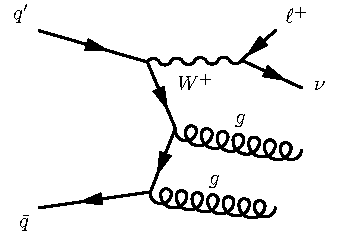
\includegraphics[width=\textwidth]{wjets}
		\caption{\label{fig:wjets}}
	\end{subfigure}
%	\begin{subfigure}[b]{0.25\linewidth}
%		\centering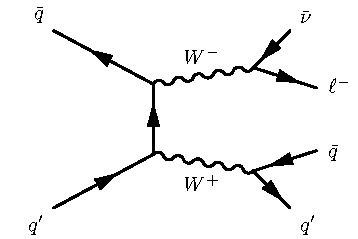
\includegraphics[width=\textwidth]{diboson}
%		\caption{\label{fig:diboson}}
%	\end{subfigure}
	\caption{Exemplary Feynman diagrams showing the dominant processes \subref{fig:ttbar} $t\bar{t}$, \subref{fig:singletop} single top and \subref{fig:wjets} $W+\textrm{jets}$ production with subsequent decays.}
	\label{fig:sm_backgrounds_feynman}
\end{figure}


\section{Monte Carlo samples}

\Cref{tab:mc_generators} summarises all \gls{mc} generators and software versions used for the simulated events used in the following. Further details are given in the relevant ATLAS simulation notes~\cite{ATL-PHYS-PUB-2018-009,ATL-PHYS-PUB-2016-005,ATL-PHYS-PUB-2017-006,ATL-PHYS-PUB-2017-005,ATL-PHYS-PUB-2016-002}.

\subsection{Signal samples}

The $\charg\neutr$ pair production signal samples were generated at \gls{lo} using \textsc{MadGraph5\_aMC@NLO} 2.6.2~\cite{MGaMCNLO:2014hca,Frederix:2012ps} with up to two additional partons in the \gls{me}. \textsc{MadGraph5\_aMC@NLO} is interfaced with \textsc{Pythia8}~\cite{Pythia8:2007gs} for the \gls{ps}, hadronisation and underlying event, using the CKKW-L~\cite{Lonnblad:2011xx} scheme for matching the \gls{ps} to the \glspl{me}. The NNPDF 2.3 LO~\cite{Ball:2012cx} \gls{PDF} set and the A14 set of tuned parameters~\cite{ATL-PHYS-PUB-2014-021} are used. For modelling the decay of \gls{hf} quarks, \textsc{EvtGen}~\cite{Lange:2001uf} v1.6 is used. 

As the $\charg/\neutr$ and $\lsp$ masses are free parameters of the signal model, they are systematically scanned, resulting in a set of 164 distinct evenly distributed in the two-dimensional grid spanned by the mass parameters. In the following the two-dimensional grid will be referred to as \textit{signal grid}, while the distinct signal scenarios (each witch a unique set of mass parameter values) will be referred to as \textit{signal point}. The generated signal grid covers $\charg/\neutr$ masses from $\SI{150}{\GeV}$ to $\SI{1.1}{\TeV}$ and $\lsp$ masses from $\SI{0}{\GeV}$ to $\SI{550}{\GeV}$, avoiding the kinematically forbidden region with $m(\charg/\neutr) < m(\lsp) + m(h)$.

Signal samples well within the expected sensitivity range of the analysis (with relatively low $\charg/\neutr$ and $\lsp$ masses) are generated using the \textsc{ATLFAST-II} detector simulation, while the full detector simulation using \textsc{Geant4} is used for the remaining model points for maximum accuracy. In order to account for pileup effects, all signal samples are overlaid with simulated minimum bias events generated using \textsc{Pythia8} and the A3 tune~\cite{ATL-PHYS-PUB-2016-017}, reweighted to match the pileup distribution measured in data. 

The cross sections for chargino pair production have been calculated using \textsc{Resummino}~\cite{Fuks:2013vua} at \gls{nlo} in the strong coupling constant and including \gls{nll} terms in the soft gluon resummation~\cite{Fiaschi:2018hgm,Fuks:2012qx}.

\subsection{Background samples}

Top pair production and single top processes were generated using \textsc{Powheg-Box} v2~\cite{PowhegBox:2010xd}, implementing the \textsc{POWHEG} method~\cite{Powheg1,Powheg2} for merging \gls{nlo} \glspl{me} with the \glspl{ps}. The \gls{ps}, hadronisation and underlying event were simulated using \textsc{Pythia8} with the A14 tune. Production of $\ttbar$ in association with a vector boson $\ttbar+V$ are generated using \textsc{MadGraph5\_aMC@NLO} 2.3.3, interfaced with \textsc{Pythia8} for the \gls{ps}. The set of \glspl{PDF} used for simulation of $\ttbar$, single top, and $\ttbar+V$ is the NNPDF2.3LO set.

Production of a vector boson $V$ with additional jets ($V+\mathrm{jets}$) is simulated using \textsc{Sherpa} 2.2.1~\cite{Gleisberg:2008ta,Bothmann:2019yzt}, allowing up to two (four) additional parton emissions at NLO (LO) accuracy. The CKKW \gls{me}+\gls{ps} matching and merging scheme~\cite{Hoeche:2009rj,Catani:2001cc}, extended to NLO accuracy~\cite{Hoeche:2012yf}. Diboson ($VV$) and multiboson ($VV$) is simulated using \textsc{Sherpa} 2.2.1 and 2.2.2. The \glspl{PDF} used are provided by the NNPDF3.0NNLO set~\cite{Ball:2014uwa} and the generator tune is the default \textsc{Sherpa} tune.

All Higgs processes are simulated using \textsc{Powheg-Box} v2 for the \gls{me} calculations and \textsc{Pythia8} for the \gls{ps}, underlying event and hadronisation. While the generation of $h+\ttbar$ uses the A14 tune and the NNPDF2.3LO set, $h+V$ and single Higgs production are simulated using the NNPDF 3.0 NNLO set and the AZNLO~\cite{ATL-PHYS-PUB-2013-017} set of tuned generator parameters.

The detector simulation for all \gls{mc} background samples was performed using the full detector simulation based on \textsc{Geant4}, introduced in \cref{sec:detector_simulation}. Except for the \gls{mc} samples generated using \textsc{Sherpa}, all background samples use \textsc{EvtGen} v1.2 or v1.6 to model the decay of \gls{hf} quarks. Similar to the signal models, all background samples are mixed with simulated minimum bias events generated with \textsc{Pythia8} and the A3 tune.

\begin{table}
	\centering
	\setlength\heavyrulewidth{0.2ex}
	\small
	\caption{Overview of configuration of \gls{mc} generators used for simulating the various signal and \gls{sm} background processes.}
	\resizebox{\textwidth}{!}{\begin{tabular} {llllll}
	\toprule
	Process & Matrix element & Parton shower & PDF set & Cross section & Tune\\ 
	\midrule
	Signal & \textsc{MadGraph5\_aMC@NLO} 2.6.2 & \textsc{Pythia} 8.230 & NNPDF 2.3 LO & NLO+NLL~\cite{Fuks:2013vua,Fiaschi:2018hgm,Fuks:2012qx} & A14 \\
	\midrule	
	$\ttbar$ & \textsc{Powheg-Box} & \textsc{Pythia} 8.230 & NNPDF2.3LO & NNLO+NNLL~\cite{Czakon:2011xx,Cacciari:2011hy} & A14 \\
	$t$ (s-channel) & \textsc{Powheg-Box} & \textsc{Pythia} 8.230 & NNPDF2.3LO & NLO~\cite{Kant:2014oha} & A14 \\
	$t$ (t-channel) & \textsc{Powheg-Box} & \textsc{Pythia} 8.230 & NNPDF2.3LO & NLO~\cite{Kant:2014oha} & A14 \\
	$t+W$ & \textsc{Powheg-Box} & \textsc{Pythia} 8.230 & NNPDF2.3LO & NNLO~\cite{Kant:2014oha,Kidonakis:2010ux,} & A14 \\
	$\ttbar + V$ & \textsc{MadGraph5\_aMC@NLO} 2.3.3 & \textsc{Pythia} 8.210 & NNPDF2.3LO & NLO~\cite{Campbell:2012dh,Lazopoulos:2008de} & A14 \\
	\midrule
	$V+\mathrm{jets}$ & \multicolumn{2}{c}{\textsc{Sherpa} 2.2.1} & NNPDF3.0NNLO & NNLO~\cite{Gavin:2010az} & \textsc{Sherpa} default \\
	$VV$ & \multicolumn{2}{c}{\textsc{Sherpa} 2.2.1/2.2.2} & NNPDF3.0NNLO & NLO~\cite{ATL-PHYS-PUB-2017-005} & \textsc{Sherpa} default\\
	$VVV$ & \multicolumn{2}{c}{\textsc{Sherpa} 2.2.1/2.2.2} & NNPDF3.0NNLO & NLO~\cite{ATL-PHYS-PUB-2017-005} & \textsc{Sherpa} default\\
	\midrule
	$h+\ttbar$ & \textsc{Powheg-Box} & \textsc{Pythia} 8.230 & NNPDF2.3LO & NLO~\cite{deFlorian:2016spz} & A14 \\
	$h+V$ & \textsc{Powheg-Box} & \textsc{Pythia} 8.212 & NNPDF3.0NNLO & NNLO~\cite{deFlorian:2016spz} & AZNLO \\
	\textit{h (ggF)} & \textsc{Powheg-Box} & \textsc{Pythia} 8.212 & NNPDF3.0NNLO & N$^3$LO+N$^3$LL~\cite{deFlorian:2016spz} & AZNLO \\
	\textit{h (VBF)} & \textsc{Powheg-Box} & \textsc{Pythia} 8.212 & NNPDF3.0NNLO & NNLO~\cite{deFlorian:2016spz} & AZNLO \\
	\bottomrule
	\end{tabular}}\vspace{3mm}
	\label{tab:mc_generators}   
\end{table}

\section{Object definitions}

The reconstruction of physics objects requires the combination of data from multiple detector components. Due to finite detector resolutions, and the sheer amount of particles produced in each collision, this process does not always work without flaws. Sometimes, objects are falsely reconstructed or not reconstructed at all. In order to minimise reconstruction errors, different identification and reconstruction criteria are introduced for each physics object category. Electrons and muons are categorised into \textit{baseline} and \textit{signal} objects. Baseline objects have a smaller purity but a higher acceptance which is \eg useful for the reconstruction of the missing transverse momentum. Stricter identification and isolation criteria are required for signal objects, resulting in lower acceptances but also lower reconstruction errors. In this analysis, signal-type objects are used as the physical objects.

\subsection{Tracks and vertices}\label{sec:reco_tracks}

The reconstruction of tracks of charged particles starts with the formation of clusters from the raw data recorded in the Pixel and \gls{sct} detectors. Clusters are formed by grouping together adjacent pixels and strips with energy deposits above threshold and are subsequently used to create three-dimensional space-points, representing the points where charged particles traversed the active \gls{id} material~\cite{PERF-2015-08}. Sets of three space-points form track seeds that serve as inputs for a combinatorial Kalman filtering technique~\cite{Fruhwirth:178627} that includes additional space-points from the remaining pixel and \gls{sct} layers to extend the preliminary trajectory. A $\chi^2$ track fit is performed at each step of the extension. Multiple track candidates are formed from seeds that can be extended by more than one compatible space-point in one layer. Ambiguities are resolved by assigning track candidates a score taking into account basic track properties like the $\chi^2$ of the track fit, or its associated $\pt$~\cite{PERF-2015-08}. The ambiguity solver requires track candidates to contain a minimum of 7 pixel and \gls{sct} clusters, have a maximum of one shared pixel cluster and two shared \gls{sct} clusters on the same layer and have no more than two holes\footnote{Holes are intersections of the track trajectory with sensitive detector material not containing a cluster.} of which only one is allows to be in the pixel detector. Track candidates also need to have $\pt > \SI{400}{\MeV}$, $\vert\eta\vert < 2.5$ and have longitudinal ($z_0$) and transversal ($d_0$) impact parameters with respect to their associated vertex satisfying $\vert z_0 \sin\theta \vert < \SI{3.0}{\milli\meter}$ and $\vert d_0 \vert < \SI{2.0}{\milli\meter}$, where $\theta$ is the polar angle of the track. Track candidates surviving the ambiguity solver are extended by compatible hits in the \gls{trt}~\cite{Cornelissen:1176900} and subject to a global high-resolution track fit before being added to the final track collection~\cite{PERF-2015-08}.

Vertex reconstruction uses a selection of tracks satisfying a set of quality requirements~\cite{ATL-PHYS-PUB-2015-026} to fit the best vertex position in a procedure iteratively downweighting less compatible tracks~\cite{PERF-2015-01}. Once the vertex position has been determined, incompatible tracks with small weights are removed and can be reused for the reconstruction of additional vertices~\cite{PERF-2015-01}. All reconstructed vertices with at least two associated tracks are kept as valid primary vertex candidates. In events with multiple candidates, the primary vertex is defined to be the one with the highest $\sum \pt^2$ of its associated tracks.

\subsection{Electrons and Photons}

Electron and photon candidates are reconstructed from energy deposits in topologically connected cells in the electromagnetic and hadronic calorimeters. The reconstruction algorithm starts with the preparation of the energy deposits into so-called \textit{topo-clusters}~\cite{PERF-2014-07}. These are formed by calorimeter cells containing energy deposits above a certain noise threshold, so-called \textit{seed} cells, including their neighbouring cells which can, in turn, also act as seed cells. All cell signals are measured at the electromagnetic scale, assuming that energy deposits stem only from electromagnetic interactions. Although the topo-clustering algorithm starts with cells from both calorimeters, only cells from the \gls{em} calorimeter are used in the subsequent electron and photon reconstruction steps. Using only \gls{em} topo-clusters with a certain threshold ratio of the \gls{em} energy to the total cluster energy significantly reduces contamination from pileup clusters~\cite{EGAM-2018-01}. The \gls{em} topo-clusters are then loosely matched to \gls{id} tracks that are re-fitted in order to account for energy losses through bremsstrahlung~\cite{EGAM-2018-01}. Vertices from photon conversions are reconstructed from tracks matched to fixed-size clusters~\cite{PERF-2017-02} and also matched to the \gls{em} topo-clusters. In the final step of the reconstruction algorithm, \gls{em} topo-clusters are sorted according to descending $E_{\mathrm{T}}$ and tested as seed clusters for dynamic, variable-size \textit{superclusters}, with different seed requirements for electrons and photons~\cite{EGAM-2018-01}. Clusters near seed candidates can be added as satellites cluster candidates, originating \eg from bremsstrahlung. Electrons and photons are then finally built from the reconstructed superclusters and their energies are calibrated using $Z\rightarrow ee$ decays~\cite{PERF-2017-03}.

The identification of prompt electrons relies on a likelihood discriminant built from quantities measured in the \gls{id} and calorimeters. The quantities are chosen according to their ability of discriminating prompt isolated electrons from non-prompt leptons originating in \gls{hf} decays, from photon conversions or from jets. They include the properties of the electron track, the shape of the \gls{em} shower and the quality of the match between the electron track and the calorimeter clusters~\cite{PERF-2017-01}. Photon identification, on the other hand, relies on a cut-based selection exploiting the shape of the \gls{em} shower.

In this analysis, electrons are required to satisfy $\pt > \SI{7}{GeV}$ and $\vert\eta\vert<2.47$. Baseline electrons are identified using the \textit{LooseAndBLayer} requirement on the identification likelihood, requiring a hit in the innermost layer of the pixel detector, at least two additional hits in the remaining layers of the pixel detector and seven hits in the pixel an \gls{sct} detectors combined~\cite{PERF-2017-01}. In addition, the longitudinal impact parameter $z_0$ of baseline electrons needs to satisfy $\Delta z_0\sin\theta < \SI{0.5}{\milli\meter}$ with respect to the primary vertex. Signal electrons are a subset of baseline electrons and need to satisfy the \textit{tight} likelihood identification, yielding an efficiency of 80\% for prompt electrons with $E_\mathrm{T}=\SI{40}{\GeV}$~\cite{PERF-2017-01}. In addition to the longitudinal impact parameter, signal leptons also need to satisfy $d_0/\sigma_{d_0} < 5$, where the transverse impact parameter $d_0$ and its uncertainty $\sigma_{d_0}$ are measured with respect to the beam line. 

Finally, electrons need to be \textit{isolated}, meaning that the vicinity of electrons needs to be clear of additional significant detector activity. Requiring electrons to be isolated prevents the selection of non-prompt electrons originating \eg from \gls{hf} decays or misidentifications of light hadrons. Isolation is quantified using two observables, one using tracking information and the other one using calorimeter data. The track based isolation variable $p_{\mathrm{T}}^{\mathrm{varcone20}}$ is the sum of all track momenta above $\SI{1}{\GeV}$, (excluding the electrons track itself) in a cone around the electron. The size of the cone is $\Delta R = \min (\SI{10}{\GeV}/\pt,0.2)$, \ie shrinking with increasing electrons $\pt$. The calorimeter based variable $E_{\mathrm{T}}^{\mathrm{cone20}}$ corresponds to the sum of the transverse energies in topo-clusters (excluding the electrons itself and after correcting for pileup effects) in a cone with $\Delta R = 0.2$ around the electrons. In this analysis, both baseline and signal electrons are required to satisfy the \textit{Loose} working point~\cite{EGAM-2018-01}, corresponding to the requirements $p_{\mathrm{T}}^{\mathrm{varcone20}}/\pt < 0.2$ and $E_{\mathrm{T}}^{\mathrm{cone20}} < 0.15$. In order improve the rejection of non-prompt electrons at high transverse momenta, electrons with $\pt >\SI{200}{\GeV}$ need to satisfy the \textit{HighPtCaloOnly} working point, applying the tighter requirement $E_{\mathrm{T}}^{\mathrm{cone20}} < \max (0.015\cdot\pt,3.5GeV)$. 

Photons are required to have $\pt > \SI{13}{GeV}$ and $\vert\eta\vert<2.37$ and need to satisfy the \textit{tight} identification and \textit{FixedCutTight} isolation requirements~\cite{EGAM-2018-01}. In this analysis, photons are only used in the calculation of the missing transverse momentum.

%\begin{table}
%	\centering
%	\setlength\heavyrulewidth{0.2ex}
%	\small
%	\caption{Overview of the object definitions for electrons.}
%	\resizebox{\textwidth}{!}{\begin{tabular} {lc}
%	\toprule
%	Selection & Value/description \\ 
%	\midrule
%	\multicolumn{2}{c}{Baseline electron} \\
%	Identification & LooseAndBLayer \\
%	$p_\mathrm{T}$ & $> \SI{7}{\GeV}$ \\
%	$\vert\eta\vert$ & $< 2.47$ \\
%	\midrule
%	\multicolumn{2}{c}{Signal electron} \\
%	\bottomrule
%	\end{tabular}}\vspace{2mm}
%	\label{tab:ele_objdef}   
%\end{table}

\subsection{Muons}

The reconstruction of muons uses primarily data from the \gls{id} and \gls{ms} and is based on the fact that muons are minimum ionising particles. Muon candidates are independently reconstructed in the \gls{id} and the \gls{ms} as muon tracks and only then combined  to a muon candidate that can be used by physics analysis~\cite{PERF-2015-10,Aad:2020gmm}. The track reconstruction in the \gls{id} follows the same procedure used for other charged-particle tracks, described in \cref{sec:reco_tracks}. In the \gls{ms}, the muon track reconstruction starts with the identification of short straight-line track segments. Segments from different \gls{ms} layers are combined into preliminary muon track candidates if they are loosely compatible with the \gls{ip} and match a first-order approximation of the parabolic trajectory describing the muon track in the magnetic field. Track candidates are then fitted in a global $\chi^2$ fit, taking into account possible \gls{ms} chamber misalignments as well as interactions with the detector material~\cite{Aad:2020gmm}. In order to increase the reconstruction performance, \gls{ms} muon tracks are subsequently combined with the \gls{id} tracks using five different reconstruction strategies, described in detail in~\cite{Aad:2020gmm}. Only two of these strategies are relevant for this analysis:
\begin{itemize}
	\item \textit{combined muons}, which are formed by combining the \gls{id} and \gls{ms} tracks through a global fit, taking into account the energy loss in the calorimeters,
	\item \textit{\gls{ms} extrapolated muons}, which are built using \gls{ms} muon tracks only, but extrapolating the tracks back to the \gls{ip} and requiring them to be loosely compatible with the \gls{ip}. Extrapolated muons are mainly used for providing acceptance in the region $2.5 < \vert\eta\vert < 2.7$, which is beyond the coverage provided by the \gls{id}.
\end{itemize}
After resolving the overlaps between the different muon types, the muon objects used for physics analysis are subject to a momentum calibration using data from $J/\Psi\rightarrow\mu\mu$ and $Z\rightarrow\mu\mu$ decays~\cite{PERF-2015-10,Aad:2020gmm}.

Identification of muons is performed using quality requirements designed to suppress non-prompt muons originating from pion and kaon decays and allow a robust momentum measurement. Muons in this analysis are built using combined and extrapolated muons that satisfy the \textit{medium} identification requirements~\cite{PERF-2015-10}. Combined muons need to have at least three hits in at least two \gls{mdt} layers, except for the region with $\vert\eta\vert < 0.1$, where a single \gls{mdt} layer is enough, as long as there is no more than one \gls{mdt} hole layer. Extrapolated muons need to have at least three hits in at least three \gls{mdt} and \gls{csc} layers. In addition, all muons need to have a significance of the ratio of the measured charge and momentum of the muons satisfying $\sigma(q/p) < 7$.

Muons in this analysis also need to satisfy $\pt > \SI{6}{\GeV}$ as well as $\vert\eta\vert < 2.7$ or $\vert\eta\vert < 2.5$ for baseline or signal muons, respectively. The longitudinal impact parameter of baseline muons is required to be $\Delta z_0\sin\theta < \SI{0.5}{\milli\meter}$ with respect to the primary vertex. Signal muons additionally need to have a transverse impact parameter satisfying $d_0/\sigma_{d_0} < 3$. Similar to electrons, muons also need to be isolated, using the same variables. Both signal and baseline muons need to conform to the \textit{Loose} working point, requiring $p_{\mathrm{T}}^{\mathrm{varcone20}}/\pt < 0.3$ and $E_{\mathrm{T}}^{\mathrm{cone20}} < 0.15$~\cite{Aad:2020gmm}.


\subsection{Jets}

\subsection{Flavour tagging}

\subsection{Missing transverse momentum}

\section{Overlap removal}

\section{Event selection}

\section{Triggers}